%%%%%%%%%%%%%%%%%%%%%%%%%%%%%%%%%%%%%%%%%%%%%%%%%%%%%%%%%%%%%%%%%%%%%%%%%%%%%%%%%%%%
%Do not alter this block of commands.  If you're proficient at LaTeX, you may include additional packages, create macros, etc. immediately below this block of commands, but make sure to NOT alter the header, margin, and comment settings here. 
\documentclass[12pt]{article}
 \usepackage[margin=1in]{geometry} 
\usepackage{amsmath,amsthm,amssymb,amsfonts, enumitem, fancyhdr, color, hyperref,comment, graphicx, environ,mathtools, bbm, tikz, setspace, cleveref,listings, dcolumn}
\usepackage{array, multirow, caption, booktabs}
\usepackage{ mathrsfs }
\usetikzlibrary{matrix,positioning}
\tikzset{bullet/.style={circle,draw=black,inner sep=8pt}}
\DeclareMathOperator*{\argmax}{arg\,max}
\DeclareMathOperator*{\argmin}{arg\,min}
\DeclareMathOperator*{\Var}{\text{Var}}
\DeclareMathOperator*{\Cov}{\text{Cov}}

\DeclarePairedDelimiter\norm{\lVert}{\rVert}%
\newtheorem{theorem}{Theorem}
\newtheorem{lemma}[theorem]{Lemma}
\DeclareMathOperator{\eps}{\varepsilon}

\DeclarePairedDelimiter\abs{\lvert}{\rvert}%
\pagestyle{fancy}
\setlength{\headheight}{65pt}
\newenvironment{problem}[2][Problem]{\begin{trivlist}
\item[\hskip \labelsep {\bfseries #1}\hskip \labelsep {\bfseries #2.}]}{\end{trivlist}}
\newenvironment{sol}
    {\emph{Solution:}
    }
    {
    \qed
    }


%%%%%%%%%%%%%%%%%%%%%%%%%%%%%%%%%%%%%%%%%%%%%%%%%%%%%%%%%%%%%%%%%%%%%%%%%%%%%%%%%


\usepackage{xcolor}
 


%%%%%%%%%%%%%%%%%%%%%%%%%%%%%%%%%%%%%%%%%%%%%

\rhead{John Higgins\\Econ 715 \\ 9 December, 2022} 

%%%%%%%%%%%%%%%%%%%%%%%%%%%%%%%%%%%%%%%%%%%%%


%%%%%%%%%%%%%%%%%%%%%%%%%%%%%%%%%%%%%%

\begin{document}
Note: I used R instead of Matlab and have included a copy of my code in the file PS2b.R! 

\begin{problem}{1}
\end{problem}
\begin{sol}
I regressed $\log(earnings)$ on education, experience, and experience squared and included the results below:
\begin{table}[!htbp] \centering 
  \caption{} 
  \label{} 
\begin{tabular}{@{\extracolsep{5pt}}lc} 
\\[-1.8ex]\hline 
\hline \\[-1.8ex] 
 & \multicolumn{1}{c}{\textit{Dependent variable:}} \\ 
\cline{2-2} 
\\[-1.8ex] & log\_earn \\ 
\hline \\[-1.8ex] 
 education & 0.151$^{***}$ \\ 
  & (0.004) \\ 
 exp & 0.059 \\ 
  & (0.066) \\ 
 exp2 & $-$0.002 \\ 
  & (0.003) \\ 
 Constant & 8.036$^{***}$ \\ 
  & (0.377) \\ 
\hline \\[-1.8ex] 
Observations & 6,134 \\ 
R$^{2}$ & 0.181 \\ 
Adjusted R$^{2}$ & 0.181 \\ 
Residual Std. Error & 0.550 (df = 6130) \\ 
F Statistic & 451.979$^{***}$ (df = 3; 6130) \\ 
\hline 
\hline \\[-1.8ex] 
\textit{Note:}  & \multicolumn{1}{r}{$^{*}$p$<$0.1; $^{**}$p$<$0.05; $^{***}$p$<$0.01} \\ 
\end{tabular} 
\end{table} 
The coefficient on education is $\beta_1 = 0.151$.
\end{sol}
\begin{problem}{2}
\end{problem}
\begin{sol}
I constructed a new dataset containing only individuals with 12 or 16 years of education. I created a treatment variable which was 1 when the individual had 16 years of education and 0 when they had 12. For each value of exp, I compute the conditional average treatment effect for each experience level and plot them below.
\begin{center}
    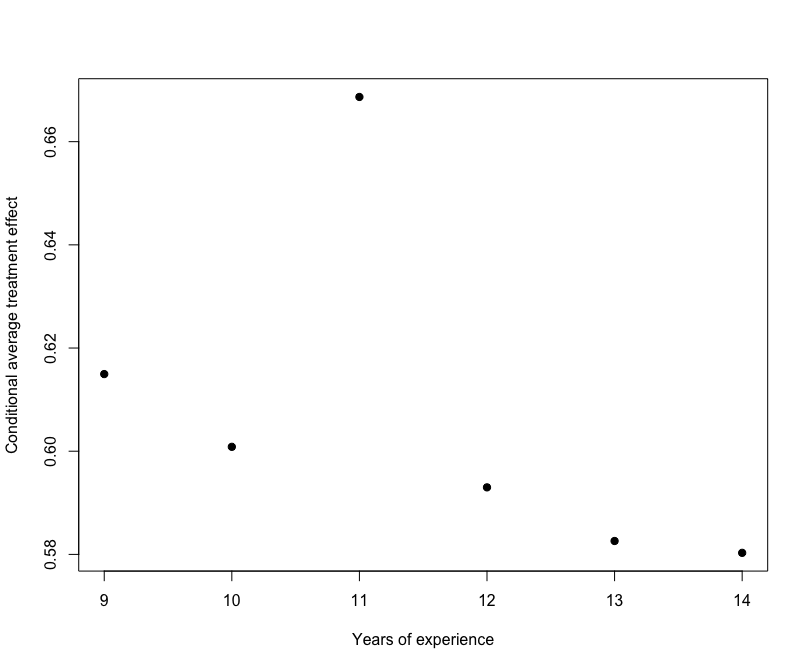
\includegraphics[scale=0.5]{CATE.png}
\end{center}

I use these to estimate the average treatment effect. I find that it is 0.6059.
\end{sol}

\begin{problem}{3}
\end{problem}
\begin{sol}
I now randomly draw a sample of size 400 from the (subsetted) data. I compute the naive average treatment effect when not controlling for experience. I find that it is 0.6049.

Furthermore, I repeat this procedure 500 times and include the histogram of estimates below (alongside with vertical lines corresponding to the estimates from problems 1 and 2):

\begin{center}
    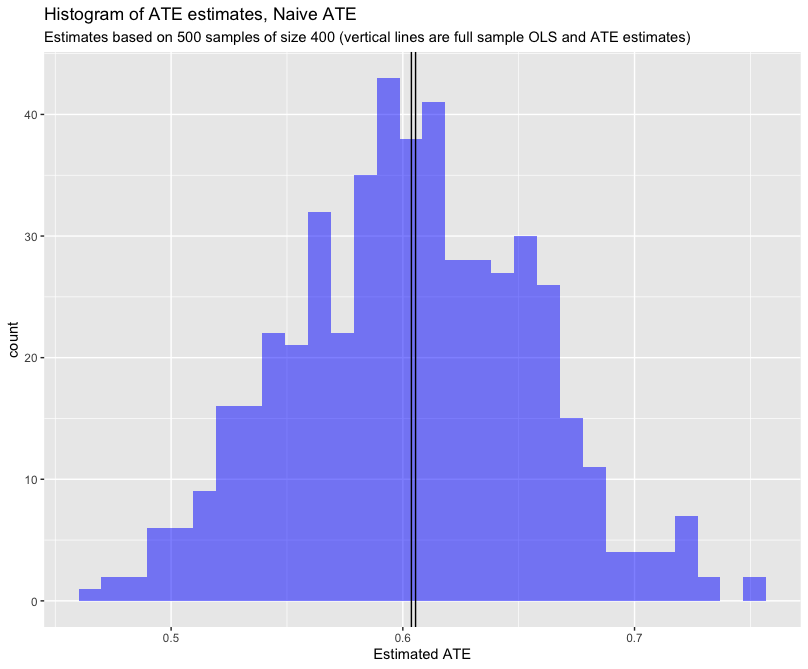
\includegraphics[scale=0.5]{Naive_hist.png}
\end{center}

I find that the mean of the naive ATE estimates is 0.6037 with a standard deviation of 0.052. The previously estimated ATEs fall pretty much in the center of this distribution.
\end{sol}

\begin{problem}{4}
\end{problem}
\begin{sol}
For this question, I use the same draw of the random sample of size 400 as was used in the previous problem. I use the treatment effect regression of $\log(earn)$ on experience and experience squared times as well as the interaction of the treatment dummy variable with each variable. This regression has the following form:
\[\log(earn) = \beta_0 + \beta_1 T + \beta_2 exp + \beta_3 exp^2 + \beta_4 T \cdot exp + \beta_5 T \cdot exp^2\]
The average treatement effect given this specification is estimated by the following:
\[\widehat{ATE} = \hat{\beta}_{1} + \hat{\beta}_4 E[exp] + \hat{\beta}_5 E[exp^2]\]
I estimate the average treatment effect to be 0.6047.

Furthermore, I repeat this procedure 500 times (using the same simulation draws as the previous question) and include the histogram of estimates below (alongside with vertical lines corresponding to the estimates from problems 1 and 2):

\begin{center}
    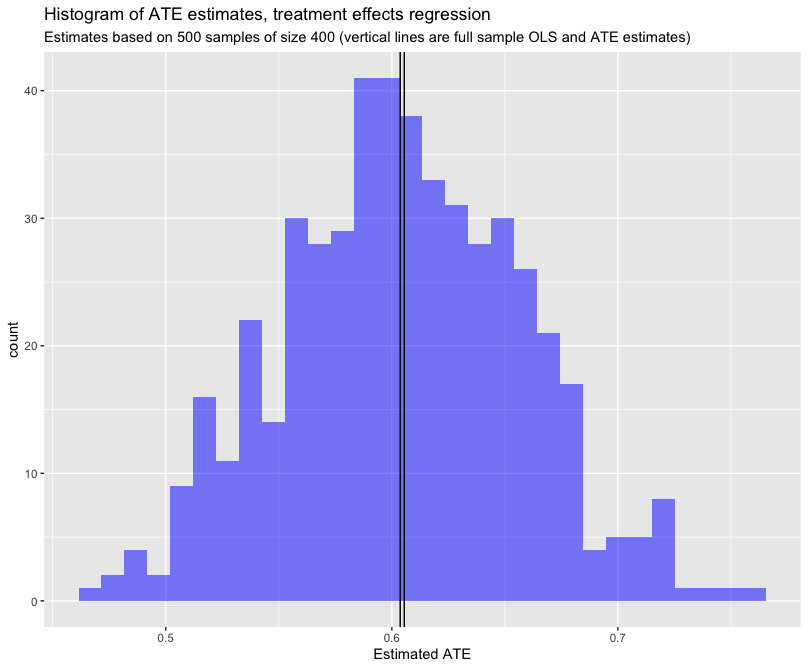
\includegraphics[scale=0.5]{Reg_hist.png}
\end{center}

I find that the mean of the regression ATE estimates is 0.6044 with a standard deviation of 0.052. The previously estimated ATEs fall very close to the center of this distribution, but seem to be slightly to the right of the peak.
\end{sol}

\begin{problem}{5}
\end{problem}
\begin{sol}
    For this question, I use the same draw of the random sample of size 400 as was used in the previous problems. Here, I use the propensity score method to estimate the average treatment effect. In this sample, I estimate the average treatment effect to be 0.6509.
    
    Furthermore, I repeat this procedure 500 times (using the same simulation draws as the previous questions) and include the histogram of estimates below (alongside with vertical lines corresponding to the estimates from problems 1 and 2):
    
    \begin{center}
        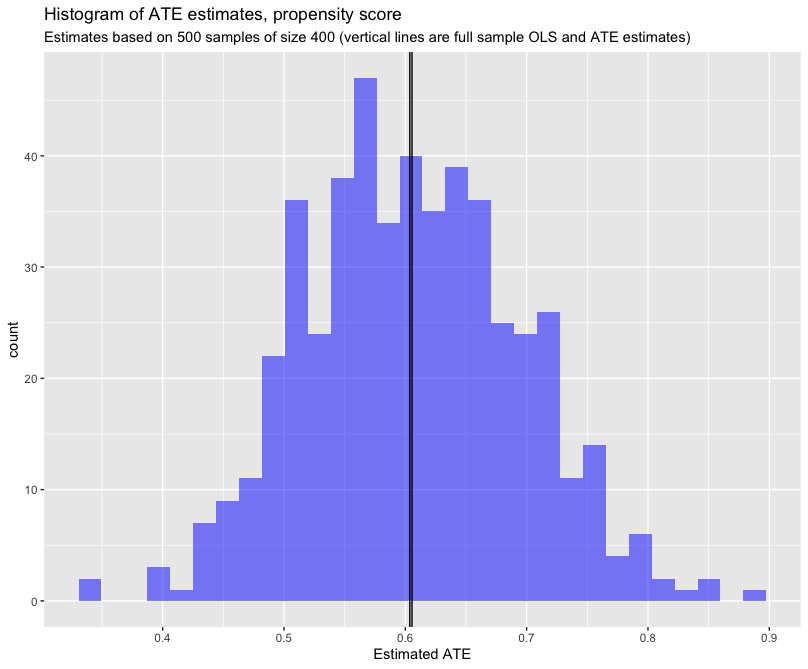
\includegraphics[scale=0.5]{Prop_hist.png}
    \end{center}
    
    I find that the mean of the regression ATE estimates is 0.6053 with a standard deviation of 0.088. As before, the previously estimated ATEs fall close to the center of this distribution.
    \end{sol}

\begin{problem}{6}
\end{problem}
\begin{sol}
The methods in problems 3,4, and 5 yield similar results overall. The mean estimates across each of the 500 draws are pretty similar (they only differ by a few to several thousandths at most). The mean of the regression estimator across 500 draws seems to be the closest to the estimate of the ATE obtained in problem 2, suggesting that this one may have the slight edge in terms of bias. The standard deviations of the naive estimator and the regression estimator are very close and are both lower than the standard deviation of the propensity score method. Since the regression estimator has lower bias overall and is tied for the lowest standard deviation, I would prefer it for this sample. It isn't surprising that this estimator gives results which are close to problem 2 since it is essentially estimating the conditional average treatment effect and then averaging across the experience levels (which is exactly what problem 2 was). 

However, these findings do not testify to the overall validity of any of the estimation strategies. For datasets with a large number of covariates, it may be a lot more reasonable to use propensity score matching (as the benefits of dimensionality reduction could far outweigh the slight inefficiency). Here, we only had two covariates (exp and exp$^2$), so the benefit of propensity score matching may be limited. We also only have 6 categories of experience, and our grouping of experience levels was a bit coarse. An approach which had more groups and/or a more sophisticated grouping procedure may offer better results.

Furthermore, in a finite sample it isn't surprising that propensity score matching may exhibit more variability: the propensity score can vary a lot across different samples, leading to higher variance in the estimated treatment effect. However, the impact of this would naturally decrease as the sample size increases. So in a large sample, propensity scores may be comparable to the other methods.
\end{sol}

\begin{problem}{7}
\end{problem}
\begin{sol}
    I used the same simulation draws for each of the three estimation procedures. My thinking was that since we are making comparisons between estimators, it is best to run the estimators on the same data so that we don't introduce the possibility of simulation error creating differences between estimators' performance. 
\end{sol}


\end{document}
